\section{Theorie}
\label{sec:Theorie}


Ein Serienresonanzkreis ist in Abbildung \ref{fig:serienreson} dargestellt.
Er besteht aus einer äußeren Spannungsquelle $U(t)$ und in Serie 
geschaltetem ohmschen Widerstand $R$, Spule mit Induktivität $L$ und Kondensator 
mit Kapazität ($\kappa$ zität) $C$ (\cite{noltingbro}).

\begin{figure}
	\centering
	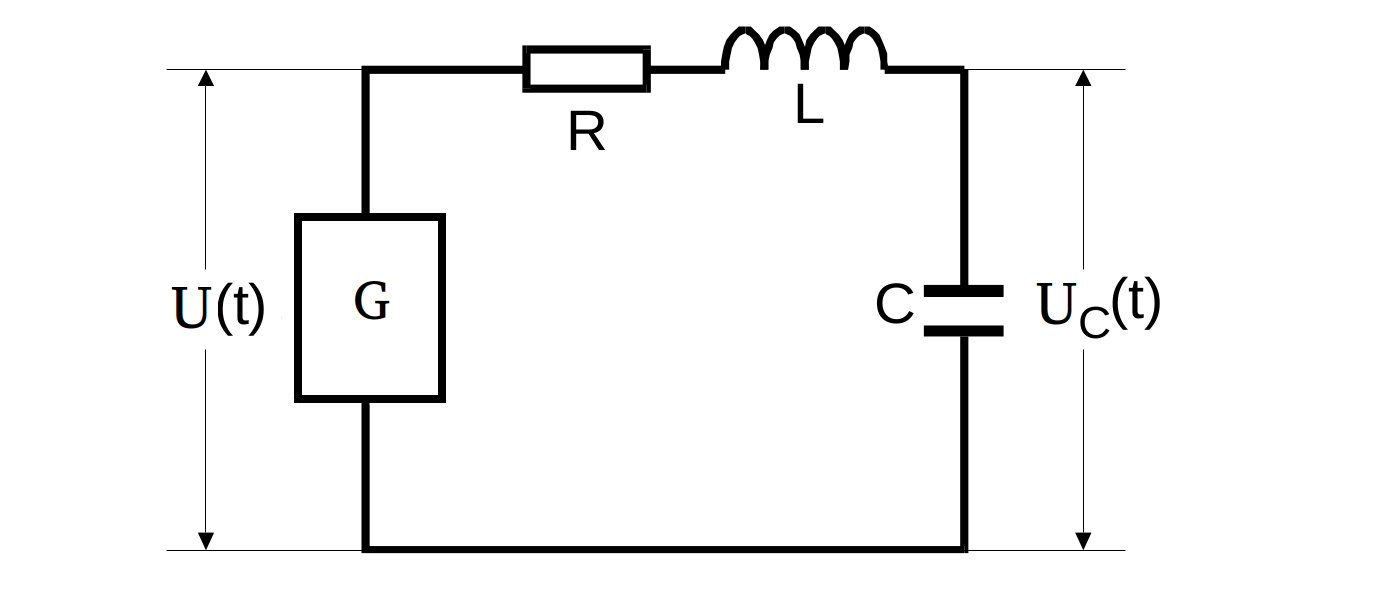
\includegraphics[width=0.7\textwidth]{Bilder/Aufbau.png}
	\caption{Schaltung eines Serienresonanzkreises \cite{Anleitung}}
	\label{fig:serienreson}
\end{figure}


\subsection{Ungedämpfte und gedämpfte Schwingungen}

Vorerst soll ein Serienresonanzkreis ohne äußere Spannungsquelle (Abbildung \ref{fig:serienresonlow}) -- also ein RLC-Kreis -- betrachtet werden.

Nimmt man an, dass zum Zeitpunkt $t=0$ ein bestimmter Energiebetrag im System vorhanden ist, 
werden elektrische Schwingungen erzeugt.
Diese lassen sich unterordnen in ungedämpfte und gedämpfte Schwingungen.

\textbf{Ungedämpfte Schwingungen} lassen sich in der Realität nicht erzeugen, da über ohmsche 
Widerstände elektrische Energie irreversibel in Wärmeenergie umgewandelt wird.
Sie entstehen also unter Vernachlässigung von ohmschen Widerständen.
Man betrachtet also einen LC-Kreis, der mit einer Spule und einem Kondensator aus zwei 
Energiespeichern besteht. 
Dann alterniert die Energie verlustfrei als elektrische bzw. magnetische Feldenergie zwischen dem Kondensator und der Spule. 
Dies ist der Fall, da bei der Entladung des Kondensators ein Magnetfeld in der Spule erzeugt 
wird, welches daraufhin abgebaut wird und wiederum zur Aufladung des Kondensators mit 
umgekehrter Polung führt. Dieser Vorgang wird periodisch fortgesetzt, sodass die Energie zwischen Spule und Kondensator oszilliert.

\textbf{Gedämpfte Schwingungen} treten hingegen auf, wenn ohmsche Widerstände nicht vernachlässigt werden. 
Dann wird nämlich teilweise die vom Strom transportierte Energie irreversibel in Wärme 
umgewandelt und die Energie im RLC-Kreis ist so nicht erhalten. Im Folgenden sollen gedämpfte 
Schwingungen näher betrachtet werden.

Mit dem 2. Kirchhoffschen Gesetz erhält man aus dem Schaltkreis in Abbildung \ref{fig:serienresonlow} die Gleichung
\begin{equation*}
	U_{\text{R}}(t) + U_{\text{C}}(t) + U_{\text{L}}(t) = 0 \text{.}
\end{equation*}
Weiterhin erhält man mit dem Ohmschen Gesetz, dem Induktionsgesetz, der Spannung $U_{\text{C}} = \frac{Q(t)}{C}$ am Kondensator und dem Zusammenhang $I = \dot{Q}$ die Differentialgleichung
\begin{equation}
	\ddot{I} + \frac{R}{L} \, \dot{I} + \frac{1}{LC} \, I = 0 \text{,}
	\label{eqn:idgl}
\end{equation}
also eine lineare, homogene Differentialgleichung 2. Ordnung.
Diese lässt sich mit dem Ansatz 
\begin{equation}
	I(t) = I_0 \, \mathrm{e}^{i \omega t}
\end{equation}
lösen, wobei $I_0, \omega \in \mathbb{C}$.
Für $\omega$ ergibt sich
\begin{equation}
	\omega_{1,2} = i \, \frac{R}{2L} \pm \sqrt{\frac{1}{LC} - \frac{R^2}{4L^2}} \text{.}
\end{equation}
Mit den Definitionen
\begin{align}
	2 \pi \mu &:= \frac{R}{2L} & 2 \pi \nu &:= \sqrt{\frac{1}{LC} - \frac{R^2}{4L^2}}
	\label{eqn:defis}
\end{align}
lässt sich die allgemeine Lösung von Gleichung \eqref{eqn:idgl} schreiben als
\begin{equation}
	I(t) = \mathrm{e}^{-2 \pi \mu t} (I_1 \mathrm{e}^{i 2 \pi \nu t} + I_2 \mathrm{e}^{-i 2 \pi \nu t}) \text{,}
\end{equation}
wobei $I_1, I_2, \nu \in \mathbb{C}$.

Nun lassen sich die drei signifikanten Fälle für $\nu$ unterscheiden in denen $\nu$ entweder reell, komplex mit $\Im \nu \neq 0$ oder verschwindet.

\subsubsection{Der Schwingfall}
Damit $\nu$ reell ist, muss der Term in der Wurzel in der zweiten Gleichung \eqref{eqn:defis} 
positiv sein, also $\frac{1}{LC} > \frac{R^2}{4L^2}$ gelten.
Ist dies der Fall, erhält man als reelle Lösungsfunktion
\begin{equation}
	I(t) = I_0 \mathrm{e}^{-2 \pi \mu t} \cos(2\pi \nu t + \eta) \text{.}
	\label{eqn:schwingi}
\end{equation}
Dieser Fall entspricht einer gedämpften Schwingung mit der Frequenz $\nu$ und der Dämpfung
durch die monoton fallende Exponentialfunktion und wird daher als Schwingfall bezeichnet.






